
%%%%% Beginning of preamble %%%%%

\documentclass[12pt]{article}  %What kind of document (article) and what size

%Packages to load which give you useful commands
\usepackage{subfig}
\usepackage{graphicx}
\usepackage{hyperref}
\usepackage{amssymb, amsmath, amsthm}

%Sets the margins

\textwidth = 6.5 in
\textheight = 9 in
\oddsidemargin = 0.0 in
\evensidemargin = 0.0 in
\topmargin = 0.0 in
\headheight = 0.0 in
\headsep = 0.0 in
\parskip = 0.2in
\parindent = 0.0in

%defines a few theorem-type environments
% \newtheorem{theorem}{Theorem}
% \newtheorem{corollary}[theorem]{Corollary}
% \newtheorem{definition}{Definition}

\newtheorem{definition}{Definition}
\newtheorem{fact}{Fact}
\newtheorem{remark}{Remark}
\newtheorem{theorem}{Theorem}
\newtheorem{proposition}{Proposition}
\newtheorem{lemma}{Lemma}
\newtheorem{corollary}{Corollary}

\renewcommand{\labelenumi}{\arabic{enumi}.}
\renewcommand{\labelenumii}{\arabic{enumi}.\arabic{enumii}.}
\renewcommand{\labelenumiii}{\arabic{enumi}.\arabic{enumii}.\arabic{enumiii}.}
\renewcommand{\labelenumiv}{\arabic{enumi}.\arabic{enumii}.\arabic{enumiii}.\arabic{enumiv}.}
\newlength{\alginputwidth}
\newlength{\algboxwidth}
\newcommand{\alginput}[1]{\makebox[1.5cm][l]{ {\sc Input:}} \parbox[t]{\alginputwidth}{{\it #1}}}
\newcommand{\algoutput}[1]{\makebox[1.5cm][l]{ {\sc Output:}} \parbox[t]{\alginputwidth}{{\it #1}}}
\newcommand{\algtitle}[1]{\underline{Algorithm \ {\bf #1}} \vspace*{1mm}\\}

%%%%% End of preamble %%%%%







\begin{document}

\title{CS150 Project 3 Report}

\author{Wah Loon Keng\\
Lafayette College, Easton, PA 18042, USA.\\
kengw{\tt @}lafayette.edu.}
\date{\today}
\maketitle

\begin{abstract}
This project is to simulate a fuel distribution network:
Given a graph with fuel depots and gas stations as vertices, with weight edges, for each station find a fuel depot to service it such that the total number of miles travelled and the longest distance from station to depot are minimized.

We present a solution by proving two lemmas\footnote{The proofs are not the most mathematically-rigorous given the time-scale of the project.}, and using them to construct the Nearest-Neighbor paths for a given graph, such that each station is guaranteed (if not isolated) service by a closest fuel depot; and the sum of the distances of all paths is minimized.

% \vspace*{5mm}
\end{abstract}











\section{Introduction} \label{intro}
{\bf Problem Statement.}\footnote{See The original problem here at Reference \ref{Problem}.} We simulate a fuel distribution network using a graph, with two types of vertices: \emph{fuel depot(depot)} and \emph{gas station(station)}, connected with undirected weighted edges.

{\bf{ The requirements are: }}
\begin{enumerate}
	\item Each station must be serviced by one and only one depot.
	\item The longest distance from any station to depot is minimized.
	\item The total distance traveled in the graph (for all paths) is minimized.
\end{enumerate}


We provide a concept named \emph{Nearest-Neighbor(NN)}, which is similar to the \emph{Nearest Neighbor Graph}\footnote{See the explanation here at Reference \ref{NNG}.}. Using \emph{NN}, we prove two lemmas of shortest path, and apply them in our solution algorithm.




\section{Approach}

\subsection{Mathematical analysis}

We define \emph{Nearest-Neighbor(NN)} on the undirected graph with two types of vertices (depots and stations) as follow: 
\begin{definition}\label{defNN}
A (connected) depot $q$ is the Nearest-Neighbor(NN) of a station $p$ if their path distance is no larger than that from $p$ to any other depot. Note that the relation is not symmetric to vertex-type.
\end{definition}

This allows us to use any shortest-path algorithm from a station, and locate the closest depot; the path can pass by other stations, and the process repeats for any unchecked stations. Since the path found is a shortest path, requirements 1, 2 are simultaneously satisfied. As the graph is undirected, we can simply reverse the path to start from depot and end at station; from now we consider the opposite.

Next, we proof two lemmas that help satisfy requirement 3:

\begin{lemma}\label{decom}
In the defined context, any decompositions of a shortest path are shortest paths.
\end{lemma}
\begin{proof}
Note that a shortest path $P$ always begins at a station $s$ and ends at a depot $d$. For the base case; the path has only two vertices, and we are done.

Suppose the path has more than two vertices. Then, decompose the path at an arbitrary vertex $v$, and call them $P1$ and $P2$, where $P = P1 \circ P2$. For the sake of contradiction, suppose $P1$ is not a shortest path from $d$ to $v$, then there must exist a shorter path $P1'$ between them, and recomposing we get $P' = P1' \circ P2$ between $(d, v)$ is shorter than the original $P$, which we assumed is the shortest. This gives the contradiction. The other part of the proof proceeds analogously.
\end{proof}


\begin{lemma}
Applying Lemma \ref{decom} to NN, once all such paths are found, and all subpaths contained within larger paths are eliminated, the resultant paths form a Nearest-Neighbor-Graph that satisfy requirement 3.
\end{lemma}
\begin{proof}
We prove only the last part via simple Riemann-Sum: the sum of minimization on all paths is the minimization on the sum of all paths. Note this also implies that Lemma 1 and 2 are metric-independent.
\end{proof}

The solution requires searching starting from stations and ending at a depot, as reflected in the asymmetry between the two types of vertices in the definition of NN. Moreover, the NNGraph takes care of loops and partially overlapping paths while satisfying requirement 3. For the project requirement 1, if a station is passed by many times, simply choose an arbitrary one to service it.

To illustrate, suppose two shortest paths overlap at some but not all parts. However, there cannot be some Hamiltonian path that substitute the overlapping part, as it would imply the existence of shortest alternative sub-paths, which contradicts Lemma \ref{decom}.


\subsection{Algorithm}

We now have the tools necessary to enumerate an algorithm:

\algtitle{Nearest-Neighbor(for undirected graph with two vertex-types)}
Given a graph,
\begin{enumerate}
	\item For each station, do a shortest-path search to a closest depot,
	\item Mark all stations traversed by the path as checked.
	\item Repeat 2-3 for any unchecked stations.
	\item From all the searched paths, select all that ends at a same depot, and 
	\item For the largest path (most vertices), scan the others(smaller, with less vertices), and eliminate any subpaths (all vertices are found in the largest path);
	\item Repeat for the next largest path down to the smallest, then add all remaining paths ending as the same depot to the NN Graph.
	\item Repeat 4-6 for any searched paths are not yet added to NN Graph.
\end{enumerate}


For the shortest-path algorithm, we use \emph{Dijkstra's algorithm}$^{\ref{Dijkstra}}$. Given a pre-built graph, if $|E|$ is the number of edges and $|V|$ is the number of vertices, the algorithm above has an estimated complexity of $\mathcal{O}(|E| + |V| Log(|V|))$ from step 1-3 using Dijkstra's, and $\mathcal{O}(|E|^2)$ from 4-7 using Insertion Sort on paths, thus the best-case estimation is 
$$\mathcal{O}(|E|^3 + |V| Log(|V|))$$
The quality of the solution depends on the choice of algorithms and specific implementation, but the general structure of our solution as supported by our analysis is sufficiently good, if not the best lower bound, in satisfying the constraints and giving the best results. 

However we have not proven that the complexity of our solution approaches the actual complexity lower bound.

This concludes the section on the assumptions, algorithm used, and quality of solution, as provided by the Lemmas.





\section{Methods}

For the implementation and testing, we first construct a generic \emph{Graph} base class with the basic structures and methods for an undirected/directed graph, and extend it to \emph{NNGraph} by adding the necessary methods for implementing our algorithm.

To handle the given input data, we construct a \emph{Importer} class. It feeds the information to a \emph{Builder} class, which builds a \emph{NNGraph} using the data and runs the algorithm. The \emph{P3} class handles all tasks by calling \emph{Builder}, builds for all the given data, and outputs the results.

\begin{enumerate}
	{\Large \item \emph{P3}}

	Calls \emph{Builder} to build from each given data the \emph{NNGraph} and outputs results.

	{\Large \item \emph{Builder}}

	Calls \emph{Importer} to obtain the necessary data for building a graph as given, then its \emph{NNGraph} by running the algorithm on the built graph. Also formats the output for project requirement.
	
	{\Large \item \emph{Importer}}

	Stores and manages the location of input data. Interprets data into stations and depots, and the corresponding shortest edges for each existing pairs of vertices.
	
	{\Large \item \emph{NNGraph}}

	The NNGraph object; has methods to run the algorithms enumerated above. Paths are simplified and stored as ArrayList of keys of nodes traversed, and path distance is recovered later when needed. The equivalent methods for the algorithm are: \emph{computeAllStations(), pollPathsOfSameDepot(), dumpSublist(), addToReducedPaths()}.


\end{enumerate}








\section{Data and Analysis}
The results for all 27 data files given are generated and exported to a text file and Mathematica for analysis.

We evaluate the result, i.e. the size and distance of the paths found, where size of a path is the number of vertices it crosses.

The manipulated variable is the graph data set, indexed from 1-27, from \emph{small-1} (and each of \emph{easy, medium, hard}, to \emph{large-3}.
The analyzed result is saved to \emph{analysis.txt}, and the path to \emph{mapping.txt}.

The format of the printed path is:
$$<depot> \ <station> \ ... \ <station> \ <path-distance>$$
All stations are searched, but isolated stations (empty paths) are not printed.


\begin{center}
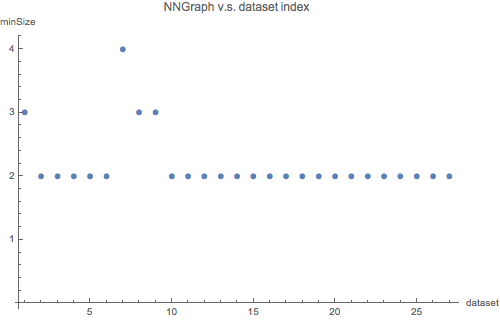
\includegraphics[scale=0.6]{p1.png}
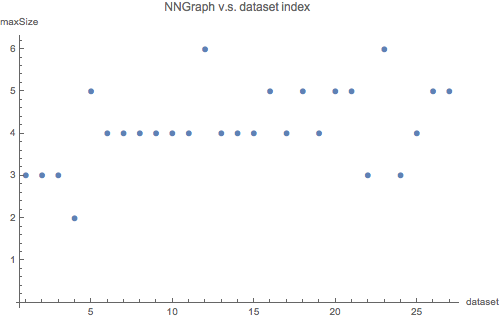
\includegraphics[scale=0.6]{p2.png}
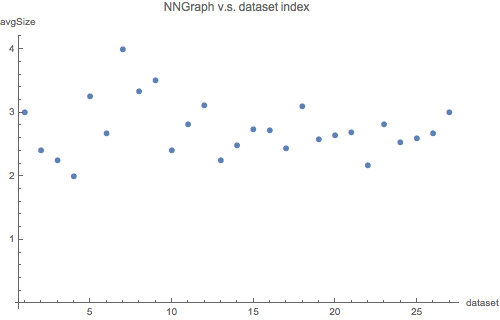
\includegraphics[scale=0.6]{p3.png}\\
{\footnotesize The plots: minimum size, maximum size, and average size of the paths found for each data set 1-27. The variation is minimal, indicating that depots are evenly distributed, and that algorithm is working as expected in yielding short paths. }
\end{center}

For the plots of minimum, maximum and average sizes, i.e. number of vertices crossed by each path, we see low variation for all data sets. The max and min differs by 2, and the average is close to 3. This indicates that depots are evenly distributed in the graph, and the algorithm is able to yield short paths, which is expected.

\begin{center}
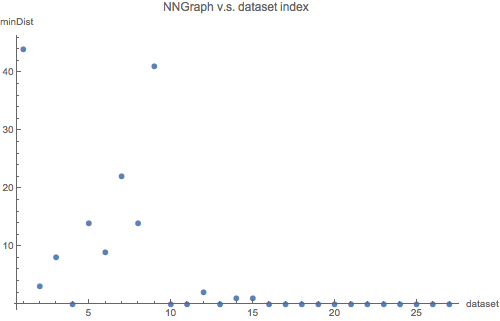
\includegraphics[scale=0.6]{p4.png}
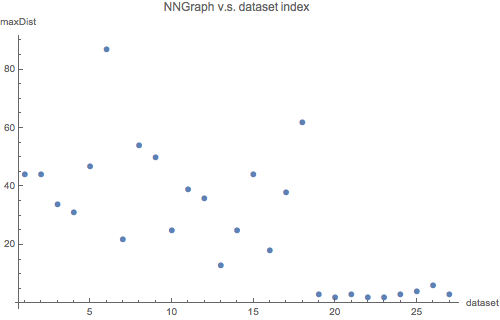
\includegraphics[scale=0.6]{p5.png}
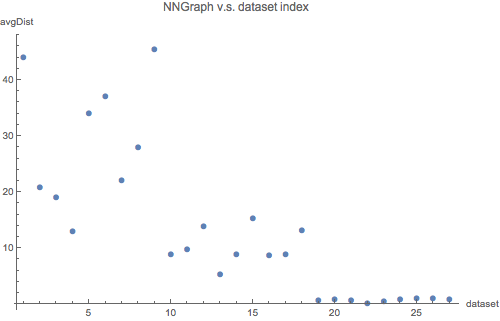
\includegraphics[scale=0.6]{p6.png}\\
{\footnotesize The plots: minimum distance, maximum distance, and average distance of the paths found for each data set 1-27. We observe slight variation: First, we see increment in distance, which is expected for harder data sets of \emph{small}. However, the distances then drop due to the input data: there's more edges with weight 0.}
\end{center}

The distance plots show some strange variation. For data set 1-9, i.e. all the \emph{small} graphs, we see the minimum varies between 0 and 50, the maximum between 10 and 90, and the average between 5 and 50. The variation is large, and since the graphs are randomly generated and of the same size, the random variation is expected.

The \emph{medium} and the \emph{big} data sets show sharp drop in distance. The behaviour is not due to errors in the algorithm or implementation, but to the original data sets. The larger randomly generated data set have more edges with zero weight in the graphs. The algorithm naturally picks up these lowest distances and yield the result, which is again expected.

Furthermore, our implementation program runs within 3 seconds for all data sets, making it sufficiently fast and practical.



\section{Conclusion}
In this project we provided a solution by defining a variation of \emph{Nearest-Neighbor Graph}. We proved two lemmas which allow us to device an algorithm that yields shortest paths from depot to stations which satisfy all three project requirements.

Moreover, we provided analysis of an implementation, showed that its performance is cool, and the result is as optimal(best) as proven by the lemmas.



\section{References}

\begin{enumerate}

\item C.W. Liew. CS150: \emph{Project III} 2014. \url{https://moodle.lafayette.edu/pluginfile.php/141173/mod_resource/content/1/p3.pdf}\label{Problem}

\item Wikipedia contributors. ``Nearest neighbor graph'' \emph{Wikipedia, The Free Encyclopedia.} 2014. \url{http://en.wikipedia.org/wiki/Nearest_neighbor_graph}\label{NNG}

\item Algolist, \emph{Dijkstra's algorithm in Java}. \url{http://www.algolist.com/code/java/Dijkstra's_algorithm}\label{Dijkstra}

\item W.L. Keng. CS150 Lab10 assignment source code: \emph{UnDirectedGraph.java} 2014.

% \item M.A. Weiss. ``Chapter 19: Binary Search Tree''. \emph{Data Structures \& Problem Solving using Java}, $4^{th}$ edition. 2010.

\item Java Platform SE 7, \emph{Class LinkedList}. \url{https://docs.oracle.com/javase/7/docs/api/java/util/LinkedList.html}

\item Java Platform SE 7, \emph{Class ArrayList}. \url{http://docs.oracle.com/javase/7/docs/api/java/util/ArrayList.html}

\item Java Platform SE 7, \emph{Class Iterator}. \url{https://docs.oracle.com/javase/7/docs/api/java/util/Iterator.html}


\end{enumerate}






\end{document} 

